% !TeX program = pdflatex
% !TeX encoding = utf8

%BEi Namensänderung des Dokuments auch die nachfolgende Zeile anpassen
% !TeX root = Vorlage.tex

%%%%%%%%%%%%%%%%%%%%%%%%%
% Dokumentinformationen %
%%%%%%%%%%%%%%%%%%%%%%%%%
\title{Vorlage}
\author{\href{mailto:lmazzole@hsr.ch}{L. Mazzoleni}}
\newcommand{\authoremail}{\href{mailto:lmazzole@hsr.ch}{lmazzole@hsr.ch} }
\newcommand{\versioninfo}{$ V1.1 $}

\documentclass[10pt,twoside,a4paper,fleqn]{scrartcl}
%%%%%%%%%%%%%%%%%%%%%%%%%%%%%%%%%%%%%%%%%%%%%
% Standard Header für 
% - Makros 
% - Farben
% - Mathematische Operatoren
\include{header/zusammenfassung}
%%%%%%%%%%%%%%%%%%%%%%%%%%%%%%%%%%%%%%%%%%%%%
%Ergänzungen für Package kommen hier hin:
%\usepackage{hyperref}


%%%%%%%%%%%%%%%%%%%%%%%%%%%%%%%%%%%%%%%%%%%%%%%%%%%%%%%%%%%%%%%%%%%%%%%%%%%%%%%%%%%%%%%%%%%%
%%%%%%%%%%%%%%%%%%%%%%%%%%%%%%%%%%%%%%%%%%%%%%%%%%%%%%%%%%%%%%%%%%%%%%%%%%%%%%%%%%%%%%%%%%%%

\begin{document}
\maketitle
\tableofcontents
\thispagestyle{empty}
\clearpage
\section*{Beispiel}
\LaTeX  hat eine gute Community $\rightarrow$ einfach Googeln

\subsection{Installation}
Infos zur Installation von \href{https://github.com/HSR-Stud/Willkommen/blob/master/installation.md#latex}{\LaTeX}, Git und \href{https://github.com/HSR-Stud/Willkommen/blob/master/installation.md#sourcetree}{Sourcetree} findet ihr hier: \url{https://github.com/HSR-Stud/Willkommen}

\subsection{Mathe Umgebung}
Texstudio Shortcut: alt + shift + m
\[ \varphi_A = \int_{A}^{Bezugspunkt}\vec{E}\cdot\vec{dl} \]

\begin{equation*}
\varphi_A = \int_{A}^{Bezugspunkt}\vec{E}\cdot\vec{dl}
\end{equation*}


\begin{equation}
    \varphi_A = \int_{A}^{Bezugspunkt}\vec{E}\cdot\vec{dl}
\end{equation}

Texstudio Shortcut: ctrl + shift + m für inline \newline
lorem $ \varphi_A = \int_{A}^{Bezugspunkt}\vec{E}\cdot\vec{dl}$ ipsum $ \varphi_A = \int_{A}^{Bezugspunkt}\vec{E}\cdot\vec{dl}$

\subsection{Bidler einfügen}
Achtung: Linux ist Casesensitiv $\rightarrow$ GrossKleinschriebung bei include Bilder beachten um kompatibilität zu gewährleisten (Wichtig mit Travis)\newline
\includegraphics[width=0.1\linewidth]{images/HSR}

\subsection{Tabelle}

    
longtable für tabellen über mehrere Seiten

%Dies ist ein Kommentar
%TODO bsp
\todo{Dies ist ein TODO}
%arraystrech verändert die "`grösse"' der Tabelle
%tabImg kann in Tabellen verwendete werden, damit das Bild nicht oben an der Tabelle klebt.
\renewcommand{\arraystretch}{2}
\begin{longtable}{| p{.25\textwidth} | p{.40\textwidth} | p{.30\textwidth} |}
    \firsthline
    \textbf{Elektrische Kraft} \newline
    \tabImg[width=3.5cm]{images/HSR} \newline {\tiny Die Kraftwirkung des geladenen Körpers (Q) auf eine elektrische Probeladung (q)}&
    \begin{equation*}\vec{F_e}(r) = \dfrac{1}{2\pi\epsilon}\cdot\dfrac{Q\cdot q}{r}\cdot\vec{r_0}\end{equation*}
    \begin{equation*}F_e(r) = \dfrac{\pi\cdot\epsilon\cdot U^2}{2\cdot r\cdot\left(ln\dfrac{r-R_1}{R_1}\right)^2}\end{equation*} & \newline
    [${F_e}$] = $\dfrac{N}{m}$\newline \newline 
    $\epsilon=\epsilon_0\cdot\epsilon_r\newline
    \widehat{=}\,${\small dielektrische Permittivität}\newline 
    $\epsilon_0 = 8.8542 \cdot 10^{-12}$ $\left[\dfrac{As}{Vm}\right]$ \newline
    $\vec{r_0}=\dfrac{\vec{r}}{|\vec{r}|}\,\widehat{=}$ Einheitsvektor \newline  
    Q, q$\,\widehat{=}\,$Linienladungsdichte$\,\left[\dfrac{C}{m}\right]$ 
    \\ \hline
    
    \textbf{Magnetische Kraft} \newline
    \tabImg[width=3.5cm]{images/HSR}   &	
    \begin{equation*}\vec{F_m}(r) = \dfrac{\mu}{2\pi}\cdot\dfrac{I\cdot i}{r}\cdot\vec{r_0} = \mu\cdot i\cdot \vec{l_0}\times\vec{H}\end{equation*} 
    \begin{equation*}F_m(r) = \dfrac{\mu\cdot I^2}{2\cdot\pi\cdot r}\end{equation*} 
    \includegraphics[width=3cm]{images/HSR}	& \newline
    $\mu =\mu_0\cdot\mu_r$\newline $\widehat{=}$ magnetische Permeabilität\newline 
    $\mu_0$ = $4\pi\cdot 10^{-7} \,\left[\dfrac{N}{A^2}\right]=\left[\dfrac{Vs}{Am}\right]$ \newline \newline
    $\vec{r_0}=\dfrac{\vec{r}}{|\vec{r}|}\,\widehat{=}$ Einheitsvektor \newline \newline 
    I, i $\widehat{=}$ elektrische Ströme 	\newline \newline 
    $[F_m]$ = $\dfrac{N}{m}$
    \\ \hline
\end{longtable}  
\resetArrayStretch

Meistens kann eine tabular-Umgebung verwendet werden. \newline
\begin{tabular}{l|r}
    Hallo & \textbf{Hallo}\\ \hline
    \textit{Hallo} & Hallo \\
\end{tabular} \qquad
\begin{tabular}{|p{7cm}|r}
    Hallo mit fixer grösse 7cm\newline
    mehrere zeilen möglich & \textbf{Hallo}\\ \hline
    \textit{Hallo} & Hallo \\
\end{tabular}

\subsection{Layout-Tipps}
\begin{minipage}{0.5\linewidth}
    \textbf{minipage} verwenden für Platzierungen.
\end{minipage}
\begin{minipage}{0.2\linewidth}
    minipage verwenden fürPplatzierungen.
\end{minipage}
\begin{minipage}{0.3\linewidth}
    minipage verwenden für Platzierungen.
\end{minipage}
\vspace{1cm}
\begin{multicols}{2}
    oder \textbf{multicols}\newline
    Lorem ipsum dolor sit amet, consetetur sadipscing elitr, sed diam nonumy eirmod tempor invidunt ut labore et dolore magna aliquyam erat, sed diam voluptua. At vero eos et accusam et justo duo dolores et ea rebum. Stet clita kasd gubergren, no sea takimata sanctus est Lorem ipsum dolor sit amet. Lorem ipsum dolor sit amet, consetetur sadipscing elitr, sed diam nonumy eirmod tempor invidunt ut labore et dolore magna aliquyam erat, sed diam voluptua. At vero eos et accusam et justo duo dolores et ea rebum. Stet clita kasd gubergren, no sea takimata sanctus est Lorem ipsum dolor sit amet.
    \columnbreak
    Lorem ipsum dolor sit amet, consetetur sadipscing elitr, sed diam nonumy eirmod tempor invidunt ut labore et dolore magna aliquyam erat, sed diam voluptua. At vero eos et accusam et justo duo dolores et ea rebum. Stet clita kasd gubergren, no sea takimata sanctus est Lorem ipsum dolor sit amet. Lorem ipsum dolor sit amet, consetetur sadipscing elitr, sed diam nonumy eirmod tempor invidunt ut labore et dolore magna aliquyam erat, sed diam voluptua. At vero eos et accusam et justo duo dolores et ea rebum. Stet clita kasd gubergren, no sea takimata sanctus est Lorem ipsum dolor sit amet.
\end{multicols}

\subsection{Spacing}
    $\backslash$qquad \newline
    $\backslash$hspace\{width\}\newline
    $\backslash$vspace\{width\}\newline
    $\backslash$newline\newline
    $\backslash$clearpage\newline
    \clearpage
\subsection{Aufzählung}
\textcolor{green}{Vorteil}:
\begin{itemize} 
    \item lineares Übertragungsverhalten
    \item einfache Ansteuerung, Drehzahleinstellung
    \item hohe Überlastfähigkeit
    \begin{enumerate}
        \item ctrl + shift + i für item
        \item ctrl + shift + i für item
    \end{enumerate}
\end{itemize}
\textcolor{red}{Nachteil}:
\begin{itemize}
    \item[><] verschleissbehaftet wegen dem mechanischen Kommutator
    \item thermische Verluste entstehen im Rotor und sind schwer abzuführen
    \item maximale Drehzahl durch mech. Kommutator begrenzt
    \begin{itemize}
        \item ctrl + shift + i für item
        \item ctrl + shift + i für item
    \end{itemize}
\end{itemize}

\section*{Einige Beispiele für die Verschiednene Packages in dieser Vorlage}
\subsection{hyperref} \label{hyperref}
Dieses Package gibt dem Benutzer nicht nur die Möglichkeit Links und Verweise innerhalb von PDF Dokumenten zu erzeugen und zu setzen, sondern auch die Änderung von Einstellungen innerhalb des PDF Dokumentes zulässt.\\
Für Verweise innerhalb eines Dokuments werden $\backslash$label\{key\} sowie die Referenz darauf mit $\backslash$ref\{key\} \ref{hyperref}, $\backslash$pageref\{key\} \pageref{hyperref} oder $\backslash$nameref\{key\} \nameref{hyperref}.\newline
Auch Links auf Websiten sind möglich wie bsp. auf \href{www.google.com}{Google}.
Weiter Infos gibt es hier:
\begin{itemize}
    \item \url{https://en.wikibooks.org/wiki/LaTeX/Labels_and_Cross-referencing}
    \item \url{https://en.wikibooks.org/wiki/LaTeX/Hyperlinks}
\end{itemize}

\subsection{circuitikz}
\url{https://de.sharelatex.com/learn/CircuiTikz_package}\newline 
\begin{circuitikz}[american voltages]
    \draw
    % rotor circuit
    (0,0) to [short, *-] (6,0)
    to [V, l_=$\mathrm{j}{\omega}_m \underline{\psi}^s_R$] (6,2) % rotor emf
    to [R, l_=$R_R$] (6,4) % rotor resistance
    to [short, i_=$\underline{i}^s_R$] (5,4) % rotor current
    
    % stator circuit
    (0,0) to [open, v^>=$\underline{u}^s_s$] (0,4) % stator voltage
    to [short, *- ,i=$\underline{i}^s_s$] (1,4) % stator current
    to [R, l=$R_s$] (3,4) % stator resistance
    to [L, l=$L_{\sigma}$] (5,4) % leakage inductance
    to [short, i_=$\underline{i}^s_M$] (5,3) % magnetizing current
    to [L, l_=$L_M$] (5,0); % magnetizing inductance
\end{circuitikz}
\\
\begin{tikzpicture}
\draw
% Thyristors leg 2
(2,0)
to[Ty] ++(0,1.5)
-- ++(0,1)
to[Ty] ++(0,1.5) coordinate (leg2)
% Thyristors leg 1
(0,0)
to[Ty] ++(0,1.5)
-- ++(0,1)
to[Ty] ++(0,1.5) coordinate (leg1)
% Connections and load RL
-- ++(2,0)
to[short, i=$i_o$, current/distance=0.5] ++(2,0)
-- ++(0,-0.8)
to[R] ++(0,-1.2)
to[L] ++(0,-1.2)
% Back to (0,0)
|- (0,0)
% AC source
(-2,1.5) coordinate (Vnn)
to[sV] ++(0,1) coordinate (Vpp)
-- (leg1 |- Vpp) node [circ] {}
(Vnn)
-- (leg2 |- Vnn) node [circ] {}
% v_o(t)
(4.5,3.5)
to[open, v^=$v_o(t)$] ++(0,-3)
;
\end{tikzpicture}

\bigskip

% Example 4-7, p. 135 of Hart, discontinuous current in full-wave rect
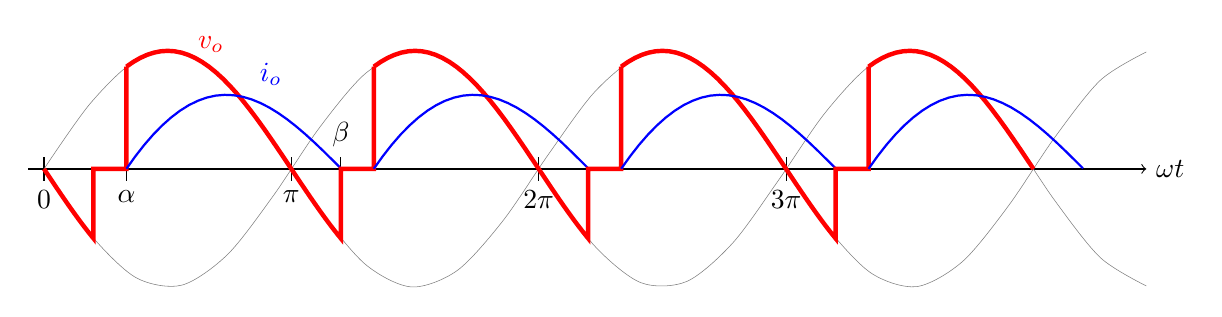
\begin{tikzpicture}
\begin{scope}[xscale=1,yscale=1.5]
\newcommand{\alphaa}{60 * pi / 180}
\newcommand{\betaa}{216 * pi / 180}

\draw[thin, ->] (-0.2, 0) -- (14,0) node[right] {$\omega t$};

\foreach \x/\xtext in {0,{\alphaa}/\alpha,{pi}/\pi,
    {\betaa}/~,{2*pi}/{2\pi},{3*pi}/{3\pi}}
\draw (\x,0.1) -- (\x,-0.1) node [below] {$\xtext$};
\draw (\betaa,-0.1) -- (\betaa,0.1) node [above] {$\beta$};


% Vs
\draw[domain=0:14, help lines, smooth]
plot (\x,{sin(\x r)});
% -Vs
\draw[domain=0:14, help lines, smooth]
plot (\x,{-sin(\x r)});
% Vo and Io
\foreach \qq [evaluate=\qq as \qqshft using \qq*pi] in {0,...,3}
{
    \begin{scope}[xshift=\qqshft cm,
    every path/.style={ultra thick, color=red}]
    % Vo
    \draw[domain=0:{\betaa-pi}]
    plot (\x,{-sin(\x r)})
    -- ({\betaa-pi},0)
    -| (\alphaa,{sin(\alphaa r)})
    [domain=\alphaa:pi]
    plot (\x,{sin(\x r)});
    % Io
    \draw
    [domain=\alphaa:\betaa,color=blue,thick]
    plot (\x,{0.05 * (13.6*sin((\x - 0.646)*180/pi)
        - 21.2*exp(-\x/0.754))});
    \end{scope}
}
\node[right,color=red] at ({pi/2+pi/12},1.05) {$v_o$};
\node[right,color=blue] at ({pi/2+pi/3},0.8) {$i_o$};
\end{scope}
\end{tikzpicture}



\subsection{rotating}
\url{https://en.wikibooks.org/wiki/LaTeX/Rotations}
\includegraphics[width=3cm]{images/HSR}
\begin{sideways}
    \includegraphics[width=3cm]{images/HSR}
\end{sideways}
\begin{turn}{30}
    \includegraphics[width=3cm]{images/HSR}
\end{turn}
\begin{rotate}{30}
    \includegraphics[width=3cm]{images/HSR}
\end{rotate}\\

\begin{table}[ht]
    \centering
    \rotatebox{30}{
        \begin{minipage}{5cm}
            \begin{tabular}{l|r}
                Hallo & \textbf{Hallo}\\ \hline
                \textit{Hallo} & Hallo \\
            \end{tabular}
        \end{minipage}
    }
    \caption{Rotated 30}
\end{table}


\subsection{hsrColor}
Verwendetes Package $\backslash$usepackage\{xcolor\} in \{header/hsrColors\}\newline
 \url{https://en.wikibooks.org/wiki/LaTeX/Colors}\newline
$\backslash$colorbox\{Farbe\}\{Text\} \hspace{1cm} \textcolor{blue}{Text}\newline
$\backslash$textcolor\{Farbe\}\{Text\} \hspace{1cm} \colorbox{red}{Text}\newline
$\backslash$fcolorbox\{Randfarbe\}\{Innenfarbe\} \hspace{1cm} \fcolorbox{red}{white}{$a^{2} + b^{2} = c^{2}$}
\begin{multicols}{4}
\fcolorbox{white}{HSRBlue}{HSRBlue}\newline
\fcolorbox{white}{HSRBlue80}{HSRBlue80}\newline
\fcolorbox{white}{HSRBlue60}{HSRBlue60}\newline
\fcolorbox{white}{HSRBlue40}{HSRBlue40}\newline
\fcolorbox{white}{HSRBlue20}{HSRBlue20}\newline\\

\fcolorbox{white}{HSRLightGray}{HSRLightGray}\newline
\fcolorbox{white}{HSRLightGray80}{HSRLightGray80}\newline
\fcolorbox{white}{HSRLightGray60}{HSRLightGray60}\newline
\fcolorbox{white}{HSRLightGray40}{HSRLightGray40}\newline
\fcolorbox{white}{HSRLightGray20}{HSRLightGray20}\newline\\


\fcolorbox{white}{HSRSchwarz}{HSRSchwarz}\newline
\fcolorbox{white}{HSRSchwarz80}{HSRSchwarz80}\newline
\fcolorbox{white}{HSRSchwarz60}{HSRSchwarz60}\newline
\fcolorbox{white}{HSRSchwarz40}{HSRSchwarz40}\newline
\fcolorbox{white}{HSRSchwarz20}{HSRSchwarz20}\newline\\

\fcolorbox{white}{HSRHematite}{HSRHematite}\newline
\fcolorbox{white}{HSRHematite80}{HSRHematite80}\newline
\fcolorbox{white}{HSRHematite60}{HSRHematite60}\newline
\fcolorbox{white}{HSRHematite40}{HSRHematite40}\newline
\fcolorbox{white}{HSRHematite20}{HSRHematite20}\newline\\

\fcolorbox{white}{HSRLakeGreen}{HSRLakeGreen}\newline
\fcolorbox{white}{HSRLakeGreen80}{HSRLakeGreen80}\newline
\fcolorbox{white}{HSRLakeGreen60}{HSRLakeGreen60}\newline
\fcolorbox{white}{HSRLakeGreen40}{HSRLakeGreen40}\newline
\fcolorbox{white}{HSRLakeGreen20}{HSRLakeGreen20}\newline\\

\fcolorbox{white}{HSRReed}{HSRReed}\newline
\fcolorbox{white}{HSRReed80}{HSRReed80}\newline
\fcolorbox{white}{HSRReed60}{HSRReed60}\newline
\fcolorbox{white}{HSRReed40}{HSRReed40}\newline
\fcolorbox{white}{HSRReed20}{HSRReed20}\newline\\

\fcolorbox{white}{HSRPetrol}{HSRPetrol}\newline
\fcolorbox{white}{HSRPetrol80}{HSRPetrol80}\newline
\fcolorbox{white}{HSRPetrol60}{HSRPetrol60}\newline
\fcolorbox{white}{HSRPetrol40}{HSRPetrol40}\newline
\fcolorbox{white}{HSRPetrol20}{HSRPetrol20}\newline\\

\fcolorbox{white}{HSRBasswood}{HSRBasswood}\newline
\fcolorbox{white}{HSRBasswood80}{HSRBasswood80}\newline
\fcolorbox{white}{HSRBasswood60}{HSRBasswood60}\newline
\fcolorbox{white}{HSRBasswood40}{HSRBasswood40}\newline
\fcolorbox{white}{HSRBasswood20}{HSRBasswood20}\newline
\end{multicols}
%\fcolorbox{white}\newline
%\fcolorbox{white}\newline
%\fcolorbox{white}\newline

\clearpage
\subsection{listings}
\url{https://en.wikibooks.org/wiki/LaTeX/Source_Code_Listings}\newline
Beispielinclude eines Matlab-Skripts mit $\backslash$lstinputlisting[style=Matlab]\{Pfad\}
\lstinputlisting[style=Matlab]{sections/Handrechnung.m}
Mögliche Styles in dieser Vorlage sind:
\begin{itemize}
    \item ASM
    \item C
    \item Cdoxy
    \item Cpp
    \item CppQT
    \item Cppunit
    \item Csharp
    \item Java
    \item Matlab
    \item R
    \item SQL
    \item VHDL
\end{itemize}


\section*{Macros}
\subsection{tabImg}
$\backslash$tabImg[arg][pfad]\\
Kann verwendet werden wie $\backslash$includegraphics[width=3cm]\{images/HSR\}.\newline
tabImg kann in Tabellen verwendete werden, damit das Bild nicht oben an der Tabelle klebt

\subsection{Verswiese auf Skript}
$\backslash$buch\{name\} \hspace{1cm} \buch{Buch}\newline
$\backslash$buchSeite\{seite\} \hspace{1cm}\buchSeite{30}\newline
$\backslash$skript\{name\} \hspace{1cm} \skript{Skript}\newline
$\backslash$formelbuch\{seite\} \hspace{1cm} \formelbuch{50}\newline

\subsection{Todos}
$\backslash$todo\{arg\} \hspace{1cm} \todo{Makros überarbeiten}
\clearpage
%%%
\input{sections/V1}
\clearpage
%%%
\section{Idiotenseite}
\subsection{Dreiecksformeln}
\begin{tabular}{lll}
	& \parbox{9.5cm}{
		\textbf{Cosinussatz} 
		\[
			c^2 = a^2 + b^2 - 2 \cdot a \cdot b \cdot \cos \gamma
		\]	
		\textbf{Sinussatz}
		\[
		\frac{a}{\sin \alpha} = \frac{b}{\sin \beta} = \frac{c}{\sin \gamma} = 2r = \frac{u}{\pi}
		\]
		\textbf{Pythagoras beim Sinus}
		\[
			\sin^2(b)+\cos^2(b)=1 \qquad \tan(b)=\frac{\sin(b)}{\cos(b)}
		\]
		}		
	& \parbox{8cm}{
		\includegraphics[width=6cm]{./idiotenseite/images/cosinussatz.png}}
\end{tabular}
\begin{center}
	\begin{multicols}{2}
		$\sin \beta = \frac ba =\frac{\text{Gegenkathete}}{\text{Hypotenuse}}$\\
		$\cos \beta = \frac ca =\frac{\text{Ankathete}}{\text{Hypotenuse}}$\\
		$\tan \beta = \frac cb =\frac{\text{Gegenkathete}}{\text{Ankathete}}$\\
		$\cot \beta = \frac cb =\frac{\text{Ankathete}}{\text{Gegenkathete}}$\\
	\end{multicols}
\end{center}

	
\subsection{Funktionswerte für Winkelargumente}
	\begin{multicols}{4}	
	\begin{tabular}[c]{|p{0.5cm}|p{0.4cm}||p{0.5cm}|p{0.5cm}|p{0.5cm}|}
	    	\hline
			deg & rad & sin & cos & tan\\
			\hline
			0\symbol{23} & 0 & 0 & 1 & 0\\
			\hline
			30\symbol{23} & $\frac{\pi}{6}$ & $\frac{1}{2}$ & $\frac{\sqrt{3}}{2}$ &
			$\frac{\sqrt{3}}{3}$\\
			\hline
			45\symbol{23} & $\frac{\pi}{4}$ & $\frac{\sqrt{2}}{2}$ & $\frac{\sqrt{2}}{2}$
			& 1\\
			\hline
			60\symbol{23} & $\frac{\pi}{3}$ & $\frac{\sqrt{3}}{2}$ & $\frac{1}{2}$ &
			$\sqrt{3}$\\
			\hline			
	\end{tabular} \\
	
	\begin{tabular}[c]{|p{0.7cm}|p{0.7cm}||p{0.7cm}|p{0.7cm}|}
	    	\hline
			deg & rad & sin & cos\\
			\hline
			90\symbol{23} & $\frac{\pi}{2}$ & 1 & 0\\
			\hline	
			120\symbol{23} & $\frac{2\pi}{3}$ & $\frac{\sqrt{3}}{2}$ & $-\frac{1}{2}$ \\
			\hline
			135\symbol{23} & $\frac{3\pi}{4}$ & $\frac{\sqrt{2}}{2}$ & $-\frac{\sqrt{2}}{2}$\\
			\hline
			150\symbol{23} & $\frac{5\pi}{6}$ & $\frac{1}{2}$ & $-\frac{\sqrt{3}}{2}$\\
			\hline
	\end{tabular} \\
	
	\begin{tabular}[c]{|p{0.7cm}|p{0.7cm}||p{0.7cm}|p{0.7cm}|}
	  	\hline
		deg & rad & sin & cos\\
		\hline
		180\symbol{23} & $\pi$ & 0 & -1\\
		\hline	
		210\symbol{23} & $\frac{7\pi}{6}$ & $-\frac{1}{2}$ & $-\frac{\sqrt{3}}{2}$\\
		\hline
		225\symbol{23} & $\frac{5\pi}{4}$ & $-\frac{\sqrt{2}}{2}$ & $-\frac{\sqrt{2}}{2}$\\
		\hline
		240\symbol{23} & $\frac{4\pi}{3}$ & $-\frac{\sqrt{3}}{2}$ & $-\frac{1}{2}$\\
		\hline
	\end{tabular} \\
	
	\begin{tabular}[c]{|p{0.7cm}|p{0.7cm}||p{0.7cm}|p{0.7cm}|}
    	\hline
		deg & rad & sin & cos\\
		\hline
		270\symbol{23} & $\frac{3\pi}{2}$ & -1 & 0\\
		\hline	
		300\symbol{23} & $\frac{5\pi}{3}$ & $-\frac{\sqrt{3}}{2}$ & $\frac{1}{2}$\\
		\hline
		315\symbol{23} & $\frac{7\pi}{4}$ & $-\frac{\sqrt{2}}{2}$ & $\frac{\sqrt{2}}{2}$\\
		\hline
		330\symbol{23} & $\frac{11\pi}{6}$ & $-\frac{1}{2}$ & $\frac{\sqrt{3}}{2}$\\
		\hline
	\end{tabular}					
\end{multicols}

\begin{minipage}{13cm}
	\subsection{Periodizität}
	$\cos(a+k\cdot2\pi)=\cos(a) \qquad \sin(a+k\cdot2\pi)=\sin(a) \qquad
	(k \in \mathbb{Z})$
	\subsection{Quadrantenbeziehungen}
	\begin{tabbing}
    	xxxxxxxxxxxxxxxxxxxxxxxxxxxxxxxxxx \= \kill
	  	$\sin(-a)=-\sin(a)$ \> $\cos(-a)=\cos(a)$\\
		$\sin(\pi - a)=\sin(a)$ \> $\cos(\pi - a)=-\cos(a)$\\
		$\sin(\pi + a)=-\sin(a)$ \> $\cos(\pi +a)=-\cos(a)$\\
		$\sin\left(\frac{\pi}{2}-a \right)=\sin\left(\frac{\pi}{2}+a \right)=\cos(a)$ \>
		$\cos\left(\frac{\pi}{2}-a \right)=-\cos\left(\frac{\pi}{2}+a \right)=\sin(a)$  
    \end{tabbing}
\end{minipage}
\begin{minipage}{5cm}
	%\begin{sidewaystable}
\subsection{Ableitungen elementarer Funktionen\formelbuch{436}}
\label{unbestimmte_integrale}
\renewcommand{\arraystretchOriginal}{2}
\begin{tabular}{|l|l||l|l|}
  \hline
  \textbf{Funktion} & \textbf{Ableitung} & \textbf{Funktion} &
  \textbf{Ableitung}\\\hline
  $C$ (Konstante) & 0 & $\sec x$ & $\dfrac{\sin x}{\cos^2 x}$ \\
  $x$ & 1 & $\sec^{-1} x$ & $\dfrac{-\cos x}{\sin^2 x}$\\
  $x^n$ ($n\in\mathbb{R}$) & $nx^{n-1}$ & $\arcsin x \quad (|x| < 1)$ &
  $\dfrac{1}{\sqrt{1-x^2}}$\\
  $\dfrac{1}{x}$ & $-\dfrac{1}{x^2}$ & $\arccos x \quad (|x| < 1)$ &
  $-\dfrac{1}{\sqrt{1-x^2}}$\\
  $\dfrac{1}{x^n}$ & $-\dfrac{n}{x^{n+1}}$ & $\arctan x$ & $\dfrac{1}{1+x^2}$\\
  $\sqrt{x}$ & $\dfrac{1}{2\sqrt{x}}$ & arccot $x$ & $-\dfrac{1}{1+x^2}$\\
  $\sqrt[n]{x}\quad (n\in\mathbb{R}, n \neq 0, x > 0)$ &
  $\dfrac{1}{n\sqrt[n]{x^{n-1}}}$ & arcsec $x$ & $\dfrac{1}{x\sqrt{x^2-1}}$\\
  $\mathrm{e}^x$ & $\mathrm{e}^x$ & arcossec $x$ & $-\dfrac{1}{x\sqrt{x^2-1}}$\\
  $\mathrm{e}^{bx}\quad (b\in\mathbb{R})$ & $b\mathrm{e}^{bx}$ & $\sinh x$ &
  $\cosh x$\\
  $a^x\quad (a > 0)$ & $a^x\ln a$ & $\cosh x$ & $\sinh x$\\
  $a^{bx}\quad (b\in\mathbb{R}, a > 0)$ & $ba^{bx}\ln a$ & $\tanh x$ &
  $\dfrac{1}{\cosh^2 x}$\\
  $\ln x$ & $\dfrac{1}{x}$ & $\coth x \quad(x \neq 0)$ & $-\dfrac{1}{\sinh^2 x}$\\
  $\log_a{x} \quad (a > 0, a \neq 1, x > 0)$ &
  $\dfrac{1}{x}\log_a{\mathrm{e}}=\dfrac{1}{x\ln a}$ & Arsinh $x$ &
  $\dfrac{1}{\sqrt{1+x^2}}$\\
  $\lg x \quad (x > 0)$ & $\dfrac{1}{x}\lg \mathrm{e}\approx \dfrac{0.4343}{x}$
  & Arcosh $x \quad (x > 1)$ & $\dfrac{1}{\sqrt{x^2-1}}$\\
  $\sin x$ & $\cos x$ & Artanh $x \quad (|x| < 1)$ & $\dfrac{1}{1-x^2}$\\
  $\cos x$ & $-\sin x$ & Arcoth $x \quad (|x| > 1)$ & $-\dfrac{1}{x^2-1}$\\
  $\tan x \quad (x\neq(2k+1)\dfrac{\pi}{2}, k\in\mathbb{Z})$ & $\dfrac{1}{\cos^2
  x}=\sec^2 x$ & $[f(x)]^n \quad (n\in\mathbb{R})$ & $n[f(x)]^{n-1}f'(x)$\\
  $\cot x \quad (x\neq k\pi, k\in\mathbb{Z})$ & $\dfrac{-1}{\sin^2 x}=-cosec^2x$ & $\ln f(x) \quad (f(x)> 0)$ & $\dfrac{f'(x)}{f(x)}$\\
  \hline
\end{tabular}
\renewcommand{\arraystretchOriginal}{1.5}
%\end{sidewaystable}
\end{minipage}
\begin{multicols}{2}
	\subsection{Additionstheoreme}
	$\sin(a \pm b)=\sin(a) \cdot \cos(b) \pm \cos(a) \cdot \sin(b)$\\
	$\cos(a \pm b)=\cos(a) \cdot \cos(b) \mp \sin(a) \cdot \sin(b)$\\	
	$\tan(a \pm b)=\dfrac{\tan(a) \pm \tan(b)}{1 \mp \tan(a) \cdot \tan(b)}$
	\columnbreak
	
	\subsection{Doppel- und Halbwinkel}	
	$\sin(2a)=2\sin(a)\cos(a)$\\
	$\cos(2a)=\cos^2(a)-\sin^2(a)=2\cos^2(a)-1=1-2\sin^2(a)$\\
	$\cos^2 \left(\frac{a}{2}\right)=\frac{1+\cos(a)}{2} \qquad
	\sin^2 \left(\dfrac{a}{2}\right)=\frac{1-\cos(a)}{2}$
\end{multicols}
\begin{multicols}{2}
	\subsection{Produkte}
		$\sin(a)\sin(b)=\frac{1}{2}(\cos(a-b)-\cos(a+b))$\\
		$\cos(a)\cos(b)=\frac{1}{2}(\cos(a-b)+\cos(a+b))$\\
		$\sin(a)\cos(b)=\frac{1}{2}(\sin(a-b)+\sin(a+b))$\\
	\subsection{Euler-Formeln} 
	$\sin(x) = \frac{1}{2j} \left(e^{jx} - e^{-jx}\right) \qquad
	\cos(x) = \frac{1}{2} \left(e^{jx} + e^{-jx}\right)$ \\
	$e^{x+jy} = e^x \cdot e^{jy} = e^x \cdot \left(\cos(y) + j\sin(y)\right)$ \\
	$e^{j\pi} = e^{-j\pi} = -1$ 
	\columnbreak
	
	\subsection{Summe und Differenz}
		$\sin(a)+\sin(b)=2 \cdot \sin \left(\frac{a+b}{2}\right) \cdot
		\cos\left(\frac{a-b}{2}\right)$\\
		$\sin(a)-\sin(b)=2 \cdot \sin \left(\frac{a-b}{2}\right) \cdot
		\cos\left(\frac{a+b}{2}\right)$\\
		$\cos(a)+\cos(b)=2 \cdot \cos \left(\frac{a+b}{2}\right) \cdot
		\cos\left(\frac{a-b}{2}\right)$\\
		$\cos(a)-\cos(b)=-2 \cdot \sin \left(\frac{a+b}{2}\right) \cdot
		\sin\left(\frac{a-b}{2}\right)$\\
		$\tan(a) \pm \tan(b)=\dfrac{\sin(a \pm b)}{\cos(a)\cos(b)}$\\
\end{multicols}

\subsection{Quellenumwandlung}
\begin{tabular}{cccp{6cm}}
Lineare Stromquelle		& $\Longleftrightarrow$ & Lineare Spannungsquelle & Formeln \\
\raisebox{-.8\totalheight}{\includegraphics[width=2.8cm]{idiotenseite/images/ersatz_strom.jpg}}&
&
\raisebox{-.8\totalheight}{\includegraphics[width=2.8cm]{idiotenseite/images/ersatz_spannung.jpg}}
&
$I_q = \frac{U_q}{R_i} = U_q \cdot G_{i Spannungsquelle}$ \newline
$U_q = \frac{I_q}{G_i} = I_q \cdot R_{i Stromquelle}$ \newline
Der Wiederstand/Leitwert bleibt gleich \newline \\
\end{tabular}
\subsection{Superposition}
\textbf{Vorgehen:}
\begin{multicols}{2}
\begin{enumerate}
  \itemsep0em
  \item Alle Quellen bis auf eine entfernen
  \item Restliche Quellen ersetzen: Stromquelle $\rightarrow$ Unterbruch,
  Spannungsquelle $\rightarrow$ Kurzschluss
  \item Teilströme mit der verbleibenden Quelle berechnen
  \item Für alle anderen Quellen das vorgehen wiederholen
  \item Alle Teilströme/-spannungen zusammenzählen
\end{enumerate}
\end{multicols}
\subsection{Einschaltvorgänge}
\subsubsection{Kondensator}
\input{idiotenseite/elektrotechnik/subsections/einschalt_kondensator}
\subsubsection{Spule}
\input{idiotenseite/elektrotechnik/subsections/einschalt_spule}


\subsection{ohmsche Leistung}
\begin{multicols}{3}
	$P=U \cdot I = I^2 \cdot R = \frac{U^2}{R}$ \\
	$P= I^2 \cdot \omega L = \frac{U^2}{\omega L}$\\
	$P= I^2 \cdot \omega C = \frac{U^2}{\omega C}$
\end{multicols}
\subsection{Strom- Spannungsquellen-Verschiebung}
\input{idiotenseite/tikz/elektrotechnik/UQuellenverschiebung1.tex}
\input{idiotenseite/tikz/elektrotechnik/UQuellenverschiebung2.tex}
\input{idiotenseite/tikz/elektrotechnik/IQuellenverschiebung1.tex}
\input{idiotenseite/tikz/elektrotechnik/IQuellenverschiebung2.tex}      
\input{idiotenseite/elektrotechnik/subsections/zeitabhaengigeGroesse}

\begin{sidewaystable}
%\begin{center}
\subsection{Allgemein zeitabhängige Grössen}
	\begin{tabular}{|ll|ll|}
    \hline
	\multicolumn{2}{|l}{Arithmetischer Mittelwert, Gleichwert, Linearer MW} 
	    	& \multicolumn{2}{l|}{$X_0 = \overline{X} = X_m = \frac {1} {T} \int\limits_{t_0}^{t_0+T}
	    	x(t)dt$} \\
	\hline
	Quadratischer MW, Leistung 
		& $X^2 = \frac {1} {T} \int\limits_{t_0}^{t_0+T} x^2(t)dt$ 
		& MW $n$. Ordnung
		& $X^n = \frac {1} {T} \int\limits_{t_0}^{t_0+T} x^n(t)dt$ \\
	\hline
	Effektivwert (RMS) 
		& $X = \sqrt{X^2} = \sqrt{\frac{1}{T} \int\limits ^{t_0+T}_{t_0}{x^2(t)dt}}$
		& Gleichrichtwert 
		& $X_{|m|} = \bar{|X|} = \frac{1}{T} \int\limits_{t_0}^{t_0+T}{|x(t)| dt}$ \\
	\hline
\end{tabular}
\vspace{0.5cm}
\subsection{Eigenschaften unterschiedlicher Schwingungsformen}

\begin{tabular}{|l|c|c|c|c|c|c|c|c|}
\hline
	Schwingungsform & Funktion & Gleichrichtwert & Formfaktor &
	Effektivwert & Crestfaktor & \textbf{$X_0$} & \textbf{$X^2$} & \textbf{var(X)} \\
\hline
	Formel &
	&
	$\overline{\left|x\right|} = \frac1T\int_{0}^{T}\left| x(t)\right|dt$&
	$\frac{X}{\overline{\left|x\right|}}$&
	$X = \sqrt{X^2} = \sqrt{\frac{1}{T} \int\limits ^{t_0+T}_{t_0}{x^2(t)dt}}$&
	$k_{s}=\frac{X_{\mathrm{max}}}{X_{\mathrm{eff}}}$&
	&
	&
	\\
\hline
	\includegraphics[width=2cm]{idiotenseite/images/table_sine_wave.png} &
	$A\cdot\sin(t)$ &
	$\frac{2}{\pi} \approx 0.637$ &
	$\frac{\pi}{2\sqrt{2}} \approx 1.11$ &
	$\frac{1}{\sqrt{2}}\approx 0.707$ &
	$\sqrt{2}\approx 1.414$ &
	$0$ &
	$\frac{A^2}{2}$ &
	$\frac{A^2}{2}$ \\
\hline	
	\includegraphics[width=2cm]{idiotenseite/images/table_full-wave_rectified_sine.png} &
	$A\cdot|\sin(t)|$ &
	$\frac{2}{\pi} \approx 0.637$ &
	$\frac{\pi}{2\sqrt{2}} \approx 1.11$ &
	$\frac{1}{\sqrt{2}} \approx 0.707$ &
	$\sqrt{2} \approx 1.414$  &
	$\frac{2A}{\pi}$ & $\frac{A^2}{2}$ & $\frac{A^2}{2}-\frac{4A^2}{\pi^2}$
	\\
\hline
	\includegraphics[width=2cm]{idiotenseite/images/table_half-wave_rectified_sine.png} &
	$\begin{cases} A\cdot\sin (t) & 0<t<\pi  \\ 0 & \textrm{somst}\end{cases}$ &
	$\frac{1}{\pi}\approx 0.318$ &
	$\frac{\pi}{2}\approx 1.571$ &
	$\frac{1}{2} = 0.5$	&
	2  &
	$\frac{A}{\pi}$ &
	$\frac{A^2}{4}$ & $\frac{A^2}{4}-\frac{A^2}{\pi^2}$
	\\
\hline
	\includegraphics[width=2cm]{idiotenseite/images/table_triangle_wave.png} &
	$A\cdot\Lambda(t)$ &
	$\frac{1}{2}= 0.5$ &
	$\frac{2}{\sqrt{3}}\approx 1.155$ &
	$\frac{1}{\sqrt{3}}
	\approx 0.557$ &
	$\sqrt{3} \approx 1.732$ &
	$0$ &
	$\frac{A^2}{3}$ &
	$\frac{A^2}{3}$ \\
\hline	
	\includegraphics[width=2cm]{idiotenseite/images/table_square_wave.png} &
	$\begin{cases} A & 0<x<t \\ 0 & \textrm{sonst}\end{cases}$ &
	$1$ &
	$1$ &
	$1$ &
	$1$ &
	$0$ &
	$A^2$ &
	$A^2$ \\
\hline	
	DC&
	1&
	$1$ &
	$1$ &
	$1$ &
	$1$  &
	-&
	-&
	-\\
\hline	
	\includegraphics[width=2cm]{idiotenseite/images/table_pulse_wide_wave.png} &
	&
	$\frac{t_1}{T}$ & $\sqrt{\frac{T}{t_1}}$ & $\sqrt{\frac{t_1}{T}}$ & $\sqrt{\frac{T}{t_1}}$ &
	$A\frac{t}{T}$ &
	$A^2\frac{t}{T}$ &
	$\frac{A^2t}{T}-\frac{A^2t^2}{T^2}$\\
\hline
\end{tabular}
%\end{center}
\end{sidewaystable}



%\subsection{Diverses}
\begin{tabbing}
	xxxxxxxxxxxxxxxxxxxxxxxxxxxx \= xxxxxxxxxxxxxxxxxxxxxxxxxxxxxx \= \kill
 	$f'(z) = \lim \limits_{\Delta z \rightarrow 0} \frac{f(z + \Delta z) -
	f(z)}{\Delta z}$ \> $(a + b)^n = \sum_{k=0}^{n} \binom n k a^{n-k} \cdot b^k$ \>
	$(a \pm b)^3 =a^3 \pm  3 a^{2} b + 3 a b^2 \pm b^3 $\\ \\
	$x_{1,2} = \dfrac{-b \pm \sqrt{b^2 - 4ac}}{2a}$ \> $\binom n k = \dfrac{n!}{k!
	\cdot (n-k)!}$ \> $(a \pm b)^4 =a^4 \pm  4 a^{3} b + 6a^2b^2 \pm 4 a b^3 +
	b^4$\\
\end{tabbing}
\subsection{Reihenentwicklungen}
\begin{tabular}{llll}
\textbf{Geometrische Reihe}
	& $\sum\limits_{n=0}^{\infty} x^n$ 
	& $= \dfrac{1}{1-x}$
	& $|x| < 1$ \\
	
	& $\sum\limits_{k=0}^{\infty} k \, x^k$ & $= x \sum\limits_{k=1}^{\infty} k \,
	x^{k-1} = \dfrac{x}{(1-x)^2} $ 
	& $x \neq 1$ \\
    & $\sum\limits_{k=0}^{n} a_0\cdot q^k$ & $= a_0 \dfrac{1-q^{n+1}}{1-q}$
    & $q \neq 1$\\
\textbf{Binominalreihe} 
	& $\sum\limits_{n=0}^\infty \binom{\alpha}{n} x^n $ &$= (1+x)^\alpha$
	& $x \in (-1,1)$ \\
\textbf{E-Funktion}
	& $\sum\limits_{k = 0}^{\infty} \dfrac{x^k}{k!}$ &$ = e^x$
	& 
\end{tabular}

\subsection{Kurven}
\begin{multicols}{4}
\subsubsection{e-Funktion}
\includegraphics[width=4.5cm]{idiotenseite/images/Exp.png}
\subsubsection{Sinus-Funktion}
\includegraphics[width=4.5cm]{idiotenseite/images/sin.png}
\subsubsection{Cosinus-Funktion}
\includegraphics[width=4.5cm]{idiotenseite/images/cos.png}
\subsubsection{Tangens-Funktion}
\includegraphics[width=4.5cm]{idiotenseite/images/tan.png}
\end{multicols}
\subsection{Idiotenformel}
Wenn ihr wissen wollt was die Formel besagt dann kauft euch doch nächstes mal
die Pro Version der Formelsammlung. Arme Schmarotzer und asoziale Personen
dürfen gerne lange darüber Rätseln was das hier soll. Aber wer zu doof ist eine
Formelsammlung ehrlich zu erwerben hat sowieso keine Chance. Haha.\\
$\frac{1}{F_{Siedlungsfl\ddot ache}}\cdot\int\limits_{\vec{x} \in
Siedlungsfl\ddot ache} \frac{1}{\int\limits_{\vec{y}\in Siedlungsfl\ddot ache\ und \left|\vec{x}-\vec{y} \right|<BH}\vec{dy}} \int\limits_{\vec{y}\in Siedlungsfl\ddot ache\ und \left|\vec{x}-\vec{y} \right|<BH} \sqrt{\frac{2\cdot\left|\vec{x}-\vec{y}\right|}{1m}+1}-1\vec{dy}\vec{dx}\frac{DSE}{m^2}$

\subsection{SI-Vorsätze}

\begin{multicols}{2}
\begin{tabular}{|l|l|l|l|}
\hline
\textbf{Symbol}	& \textbf{Name} & \textbf{Wert} & \textbf{Binär} \\
\hline
da	& Deka 	& $10^1$ & \\
\hline
h	& Hekto & $10^2$ & \\ 
\hline
k	& Kilo	& $10^3$ & $2^{10} = 1024$ \\
\hline
M	& Mega	& $10^6$ & $2^{20}$\\
\hline
G	& Giga  & $10^9$ & $2^{30}$\\
\hline
T	& Tera	& $10^{12}$ & $2^{40}$ \\
\hline
P	& Peta	& $10^{15}$ & $2^{50}$\\
\hline
\end{tabular}

\columnbreak

\begin{tabular}{|l|l|l|}
\hline
\textbf{Symbol}	& \textbf{Name} & \textbf{Wert} \\
\hline
d	& Dezi	& $10^{-1}$ \\
\hline
c	& Centi	& $10^{-2}$ \\ 
\hline
m	& Milli	& $10^{-3}$ \\
\hline
y, $\mu$ & Mikro & $10^{-6}$ \\
\hline
n	& Nano	& $10^{-9}$ \\
\hline
p	& Piko	& $10^{-12}$ \\
\hline
f	& Femto & $10^{-15}$ \\
\hline
\end{tabular}
\end{multicols}
\subsection{Griechisches Alphabet}
\begin{multicols}{2}
	\subsubsection{klein}
	\begin{tabular}{ |l|l|l|l|l|l|l|l|}
		\hline
		$\alpha$&Alpha&$\theta$&Theta&o&o&$\tau$&Tau\\
		\hline
		$\beta$&Beta&$\vartheta$&Theta&$\pi$&Pi&$\upsilon$&Ypsilon\\
		\hline
		$\gamma$&Gamma&$\gamma$&Gamma&$\varpi$&Pi&$\phi$&Phi\\
		\hline
		$\delta$&Delta&$\kappa$&Kappa&$\rho$&Roh&$\varphi$&Phi\\
		\hline
		$\epsilon$&Epsilon&$\lambda$&Lambda&$\varrho$&Roh&$\chi$&Chi\\
		\hline
		$\varepsilon$&Epsilon&$\mu$&Mu&$\sigma$&Sigma&$\psi$&Psi\\
		\hline
		$\zeta$&Zeta&$\nu$&Nu&$\varsigma$&Sigma&$\omega$&Omega\\
		\hline
		$\eta$&Eta&$\xi$&Xi&&&&\\
		\hline
	\end{tabular}
	\columnbreak
	
	\subsubsection{gross}
	\begin{tabular}{|l|l|l|l|l|l|l|l|}
		\hline
		$\Gamma$&Gamma&$\Lambda$&Lambda&$\Sigma$&Sigma&$\Psi$&Psi\\
		\hline
		$\Delta$&Delta&$\Xi$&Xi&$\Upsilon$&Ypsilon&$\Omega$&Omega\\
		\hline
		$\Theta$&Theta&$\Pi$&Pi&$\Phi$&Phi&&\\
		\hline
	\end{tabular}
\end{multicols}
\begin{sidewaystable}
\subsection{Einige unbestimmte Integrale\formelbuch{1074}}
\label{unbestimmte_integrale}
\begin{tabular}{|p{12cm}|p{13cm}|}
  \hline
  
    $ \int dx=x+C $ &
     $ \int{x^\alpha}dx=\frac{x^{\alpha+1}}{\alpha+1}+C,\ x \epsilon \mathbb
    R ^+,\ \alpha \epsilon \mathbb R \backslash \{ -1 \} $ \\\hline
     $ \int{\frac{1}{x}}dx=\ln \left| x \right| + C,\ x\neq0 $ &
     $ \int{e^x}dx=e^x+C $ \\\hline
     $ \int{a^x}dx=\frac{a^x}{\ln{a}}+C,\ a \epsilon \mathbb 
    R^+\backslash\{1\} $ &
     $ \int{ \sin{x}} dx = -\cos{x} + C $ \\\hline
     $ \int{\cos{x}} dx = \sin{x} + C $ &
     $ \int{\frac{dx}{\sin^2x}}=-\cot{x}+C,\ x\neq k\pi\ \mathrm{mit}\ k
    \epsilon \mathbb Z $ \\\hline
     $ \int{\frac{dx}{\cos^2x}}=\tan{x}+C,\ x\neq\frac{\pi}{2}+k\pi\
    \mathrm{mit} k \epsilon \mathbb Z $ & 
    
    %10. :
     $ \int{\sinh{x}}dx = \cosh{x}+C $ \\ \hline
     $ \int{\cosh{x}}dx = \sinh{x}+C $ &
     $ \int{\frac{dx}{\sinh^2x}}=-\coth{x}+C,\ x\neq0 $ \\\hline
     $ \int{\frac{dx}{\cosh^2x}}=\tanh{x}+C $ &
     $ \int{\frac{dx}{ax+b}} = \frac{1}{a}\ln \left|ax + b\right| + C,\
    a\neq 0,x\neq-\frac{b}{a} $ \\\hline
     $ \int{\frac{dx}{a^2x^2+b^2}}=\frac{1}{ab}\arctan{\frac{a}{b}x}+C,\
    a\neq0,\ b\neq0 $ &
     $
    \int{\frac{dx}{a^2x^2-b^2}}=\frac{1}{2ab}\ln{\left|\frac{ax-b}{ax+b}\right|}+C,\
    a\neq0,\ b\neq0,\ x\neq\frac{b}{a},\ x\neq-\frac{b}{a} $ \\\hline
     $
    \int{\sqrt{a^2x^2+b^2}}dx=\frac{x}{2}\sqrt{a^2x^2+b^2}+\frac{b^2}{2a}\ln{(ax+\sqrt{a^2x^2+b^2})}+C,\
    a\neq0,\ b\neq0 $ &
     $
    \int{\sqrt{a^2x^2-b^2}}dx=\frac{x}{2}\sqrt{a^2x^2-b^2}-\frac{b^2}{2a}\ln\left|ax+\sqrt{a^2x^2-b^2}\right|+C,\
    a\neq0,\ b\neq0,a^2x^2\geqq b^2$ \\\hline
     $
    \int\sqrt{b^2-a^2x^2}dx=\frac{x}{2}\sqrt{b^2-a^2x^2}+\frac{b^2}{2a}\arcsin\frac{a}{b}x+C,\
    a\neq0,\ b\neq0,\ a^2x^2\leqq b^2 $ &
    %20.:
     $
    \int\frac{dx}{\sqrt{a^2x^2-b^2}}=\frac{1}{a}\ln(ax+\sqrt{a^2x^2+b^2})+C,\
    a\neq0,\ b\neq0 $ \\\hline
     $
    \int\frac{dx}{\sqrt{a^2x^2-b^2}}=\frac{1}{a}\ln\left|ax+\sqrt{a^2x^2-b^2}\right|+C,\
    a\neq0,\ b\neq0,\ a^2x^2>b^2 $ &
     $ \int\frac{dx}{\sqrt{b^2-a^2x^2}}=\frac{1}{a}\arcsin\frac{a}{b}x+C,\
    a\neq0,\ b\neq0,\ a^2x^2<b^2 $ \\\hline
     Die Integrale $\int\frac{dx}{X}, \int\sqrt{X}dx,
    \int\frac{dx}{\sqrt{X}}$ mit $X=ax^2+2bx+c,\ a\neq0 $ werden durch 
    die Umformung $X=a(x+\frac{b}{a})^2+(c-\frac{b^2}{a}) $ und die
    Substitution $ t=x+\frac{b}{a} $ in die oberen 4 Zeilen
    transformiert. & $ \int\frac{xdx}{X}=\frac{1}{2a}\ln\left|X\right|-\frac{b}{a}\int\frac{dx}{X},\
    a\neq0,\ X=ax^2+2bx+c $ \\\hline
     $ \int\sin^2axdx=\frac{x}{2}-\frac{1}{4a}\cdot\sin2ax+C,\ a\neq0 $ &
     $ \int\cos^2axdx=\frac{x}{2}+\frac{1}{4a}\cdot\sin2ax+C,\ a\neq0 $ \\\hline
     $ \int\sin^naxdx=-\frac{sin^{n-1}ax\cdot\cos
    ax}{na}+\frac{n-1}{n}\int\sin^{n-2}axdx,\ n \epsilon \mathbb N,\ a\neq0 $ &
     $ \int\cos^naxdx=\frac{\cos^{n-1}ax\cdot\sin
    ax}{na}+\frac{n-1}{n}\int\cos^{n-2}axdx,\ n\epsilon \mathbb N,\ a\neq0 $
    \\\hline
     $ \int\frac{dx}{\sin ax} =
    \frac{1}{a}\ln\left|\tan\frac{ax}{2}\right|+C,\ a\neq0,\ x\neq
    k\frac{\pi}{a}\ \mathrm{mit}\ k\epsilon\mathbb Z$ &
    %30.:
     $ \int\frac{dx}{\cos
    ax}=\frac{1}{a}\ln\left|\tan(\frac{ax}{2}+\frac{\pi}{4})\right|+C,\ a\neq0,\
    x\neq\frac{\pi}{2a}+k\frac{\pi}{a}\ \mathrm{mit}\ k\epsilon\mathbb Z $
    \\\hline
     $\int\tan axdx=-\frac{1}{a}\ln\left|\cos ax\right|+C,\ a\neq0,\
    x\neq\frac{\pi}{2a}+k\frac{\pi}{a} \mathrm{mit}\ k\epsilon\mathbb Z$ &
     $\int\cot axdx=\frac{1}{a}\ln\left|\sin ax\right|+C,\ a\neq0,\ x\neq
    k\frac{\pi}{a} \mathrm{mit} k\epsilon\mathbb Z $ \\ \hline
     $ \int x^n\sin axdx=-\frac{x^n}{a}\cos ax+\frac{n}{a}\int x^{n-1}\cos
    axdx,\ n\epsilon\mathbb N,\ a\neq0 $ &
    $ \int x^n\cos axdx=\frac{x^n}{a}\sin ax-\frac{n}{a}\int x^{n-1}\sin
    axdx,\ n\epsilon\mathbb N,\ a\neq0 $ \\ \hline
     $ \int x^ne^{ax}dx=\frac{1}{a}x^ne^{ax}-\frac{n}{a}\int
    x^{n-1}e^{ax}dx,\ n\epsilon\mathbb N,\ a\neq0 $ &
     $ \int e^{ax}\sin bxdx=\frac{e^{ax}}{a^2+b^2}(a\sin bx-b\cos bx)+C,\
    a\neq0,\ b\neq0 $  \\ \hline
     $ \int e^{ax}\cos bxdx=\frac{e^{ax}}{a^2+b^2}(a\cos bx + b\sin bx)+C,\
    a\neq0,\ b\neq0 $ &
     $ \int\ln x dx = x(\ln x-1)+C,\ x\epsilon\mathbb R^+ $ \\ \hline
     $ \int x^\alpha \cdot \ln xdx =
    \frac{x^{\alpha+1}}{(\alpha+1)^2}\lbrack(\alpha+1)\ln x-1\rbrack + C,\
    x\epsilon\mathbb R^+,\ \alpha\epsilon\mathbb R\backslash\{-1\} $ & \\ \hline
    %FF1 Seite 496
    
\end{tabular}
\end{sidewaystable}
%\begin{sidewaystable}
\subsection{Ableitungen elementarer Funktionen\formelbuch{436}}
\label{unbestimmte_integrale}
\renewcommand{\arraystretchOriginal}{2}
\begin{tabular}{|l|l||l|l|}
  \hline
  \textbf{Funktion} & \textbf{Ableitung} & \textbf{Funktion} &
  \textbf{Ableitung}\\\hline
  $C$ (Konstante) & 0 & $\sec x$ & $\dfrac{\sin x}{\cos^2 x}$ \\
  $x$ & 1 & $\sec^{-1} x$ & $\dfrac{-\cos x}{\sin^2 x}$\\
  $x^n$ ($n\in\mathbb{R}$) & $nx^{n-1}$ & $\arcsin x \quad (|x| < 1)$ &
  $\dfrac{1}{\sqrt{1-x^2}}$\\
  $\dfrac{1}{x}$ & $-\dfrac{1}{x^2}$ & $\arccos x \quad (|x| < 1)$ &
  $-\dfrac{1}{\sqrt{1-x^2}}$\\
  $\dfrac{1}{x^n}$ & $-\dfrac{n}{x^{n+1}}$ & $\arctan x$ & $\dfrac{1}{1+x^2}$\\
  $\sqrt{x}$ & $\dfrac{1}{2\sqrt{x}}$ & arccot $x$ & $-\dfrac{1}{1+x^2}$\\
  $\sqrt[n]{x}\quad (n\in\mathbb{R}, n \neq 0, x > 0)$ &
  $\dfrac{1}{n\sqrt[n]{x^{n-1}}}$ & arcsec $x$ & $\dfrac{1}{x\sqrt{x^2-1}}$\\
  $\mathrm{e}^x$ & $\mathrm{e}^x$ & arcossec $x$ & $-\dfrac{1}{x\sqrt{x^2-1}}$\\
  $\mathrm{e}^{bx}\quad (b\in\mathbb{R})$ & $b\mathrm{e}^{bx}$ & $\sinh x$ &
  $\cosh x$\\
  $a^x\quad (a > 0)$ & $a^x\ln a$ & $\cosh x$ & $\sinh x$\\
  $a^{bx}\quad (b\in\mathbb{R}, a > 0)$ & $ba^{bx}\ln a$ & $\tanh x$ &
  $\dfrac{1}{\cosh^2 x}$\\
  $\ln x$ & $\dfrac{1}{x}$ & $\coth x \quad(x \neq 0)$ & $-\dfrac{1}{\sinh^2 x}$\\
  $\log_a{x} \quad (a > 0, a \neq 1, x > 0)$ &
  $\dfrac{1}{x}\log_a{\mathrm{e}}=\dfrac{1}{x\ln a}$ & Arsinh $x$ &
  $\dfrac{1}{\sqrt{1+x^2}}$\\
  $\lg x \quad (x > 0)$ & $\dfrac{1}{x}\lg \mathrm{e}\approx \dfrac{0.4343}{x}$
  & Arcosh $x \quad (x > 1)$ & $\dfrac{1}{\sqrt{x^2-1}}$\\
  $\sin x$ & $\cos x$ & Artanh $x \quad (|x| < 1)$ & $\dfrac{1}{1-x^2}$\\
  $\cos x$ & $-\sin x$ & Arcoth $x \quad (|x| > 1)$ & $-\dfrac{1}{x^2-1}$\\
  $\tan x \quad (x\neq(2k+1)\dfrac{\pi}{2}, k\in\mathbb{Z})$ & $\dfrac{1}{\cos^2
  x}=\sec^2 x$ & $[f(x)]^n \quad (n\in\mathbb{R})$ & $n[f(x)]^{n-1}f'(x)$\\
  $\cot x \quad (x\neq k\pi, k\in\mathbb{Z})$ & $\dfrac{-1}{\sin^2 x}=-cosec^2x$ & $\ln f(x) \quad (f(x)> 0)$ & $\dfrac{f'(x)}{f(x)}$\\
  \hline
\end{tabular}
\renewcommand{\arraystretchOriginal}{1.5}
%\end{sidewaystable}



\end{document}
